% Usage: knitr slide


\def\apacue{1}
\chapter{Introduction to the \R\ \co{rms} Package:
  The Linear Model}\alabel{chap:rmsintro}
Some of the purposes of the \co{rms} package are to
\bi
\item make everyday statistical modeling easier to do
\item make modern statistical methods easy to incorporate into everyday work
\item make it easy to use the bootstrap to validate models
\item provide ``model presentation graphics''
\ei
  
\section{Formula Language and Fitting Function}%\sound{rrms-1}
\bi
\item Statistical formula in S:
\begin{Schunk}
\begin{Sinput}
y ~ x1 + x2 + x3
\end{Sinput}
\end{Schunk}
\co{y} \emph{is modeled as} $\alpha + \beta_{1}x_{1} + \beta_{2}x_{2}
+ \beta_{3} x_{3}$.
\item \co{y} is the dependent variable/response/outcome, \co{x}'s are
  predictors (independent variables)
\item The formula is the first argument to a \emph{fitting}
  function (just as it is the first argument to a \co{trellis}
  graphics function)
\item \co{rms} (\emph{regression modeling strategies}) package~\cite{rrms}
  makes many aspects of regression modeling
  and graphical display of model results easier to do
\item \co{rms} does a lot of bookkeeping to
  remember details about the \emph{design matrix} for the model and to
  use these details in making automatic hypothesis tests, estimates,
  and plots.  The design matrix is the matrix of independent variables
  after coding them numerically and adding nonlinear and product terms
  if needed.
\item \co{rms} package fitting function for ordinary least squares
  regression (what is often called the \emph{linear model} or
  \emph{multiple linear regression}): \co{ols}
\item Example:\ipacue
\begin{Schunk}
\begin{Sinput}
f <- ols(y ~ age + sys.bp, data=mydata)
\end{Sinput}
\end{Schunk}
\item \co{age} and \co{sys.bp} are the two predictors (independent
variables) assumed to have linear and additive effects (do not
interact or have synergism)
\item \co{mydata} is an \R\ \emph{data frame} containing at least
  three columns for the model's variables
\item \co{f} (the \emph{fit object}) is an \R\ list object, containing
  coefficients, variances, and many other quantities
\item Below, the fit object will be \co{f} throughout.  In practice,
  use any legal \R\  name, e.g. \co{fit.full.model}
\ei

\section{Operating on the Fit Object}%\sound{rrms-2}
\bi
\item Regression coefficient estimates may be obtained by any of the
  methods listed below
\begin{Schunk}
\begin{Sinput}
f$coefficients
f$coef          # abbreviation
coef(f)         # use the coef extractor function
coef(f)[1]      # get intercept
f$coef[2]       # get 2nd coefficient (1st slope)
f$coef['age']   # get coefficient of age
coef(f)['age']  # ditto
\end{Sinput}
\end{Schunk}
\item But often we use \emph{methods} which do something more
  interesting with the model fit.
 \begin{description}
 \item[\co{print(f)}]: print coefficients, standard errors, $t$-test,
   other statistics; can also just type \co{f} to print
 \item[\co{fitted(f)}]: compute $\hat{y}$
 \item[\co{predict(f, newdata)}]: get predicted values, for subjects
   described in data frame \co{newdata}\footnote{You can get
     confidence limits for predicted means or predicted individual
     responses using the \co{conf.int} and \co{conf.type} arguments to
     \co{predict}.  \co{predict(f)} without the \co{newdata} argument
     yields the same result as \co{fitted(f)}.}
 \item[\co{r <- resid(f)}]: compute the vector of $n$ residuals
   (here, store it in \co{r})
 \item[\co{formula(f)}]: print the regression formula fitted
 \item[\co{anova(f)}]: print ANOVA table for all total and partial
   effects
 \item[\co{summary(f)}]: print estimates partial effects using
   meaningful changes in predictors
 \item[\co{Predict(f)}]: compute predicted values varying a few
   predictors at a time (convenient for plotting)
 \item[\co{ggplot(p)}]: plot partial effects, with predictor ranging
   over the $x$-axis, where \co{p} is the result of \co{Predict}
 \item[\co{g <- Function(f)}]: create an \R\ function that
   evaluates the analytic form of the fitted function
 \item[\co{nomogram(f)}]: draw a nomogram of the model
 \end{description}
\ei

\section{The \co{rms} \co{datadist} Function}%sound{rrms-3}%
\ipacue
To use \co{Predict, summary}, or \co{nomogram} in the \co{rms}
  package, you need to let \co{rms} first compute summaries of the
  distributional characteristics of the predictors:
\begin{Schunk}
\begin{Sinput}
dd <- datadist(x1,x2,x3,...)   # generic form
dd <- datadist(age, sys.bp, sex)
dd <- datadist(mydataframe)    # for a whole data frame
options(datadist='dd')         # let rms know where to find
\end{Sinput}
\end{Schunk}
Note that the name \co{dd} can be any name you choose as long as you
use the same name in quotes to \co{options} that you specify
(unquoted) to the left of <- \co{datadist(...)}.  It is best to
invoke \co{datadist} early in your program before fitting any
models.  That way the \co{datadist} information is stored in the fit
  object so the model is self-contained.  That allows you to make
  plots in later sessions without worrying about \co{datadist}.  \\
\co{datadist} must be re-run if you add a new predictor or recode an
old one.  You can update it using for example
\begin{Schunk}
\begin{Sinput}
dd <- datadist(dd, cholesterol, height)
# Adds or replaces cholesterol, height summary stats in dd
\end{Sinput}
\end{Schunk}

\section{Short Example}\alabel{sec:rmsintro-leadcontinuous}\ipacue\sound{rrms-4}
Consider the lead exposure dataset from B.\ Rosner \emph{Fundamentals
  of Biostatistics} and originally from Landrigan PJ~\emph{et al}, Lancet
1:708-715, March 29, 1975.  The study was of psychological and
neurologic well-being of children who lived near a lead smelting
plant.  The primary outcome measures are the Wechsler full-scale IQ
score (\co{iqf}) and the finger-wrist tapping score \co{maxfwt}.  The
dataset is available at \url{biostat.mc.vanderbilt.edu/DataSets}
and can be automatically downloaded and \co{load()}'d into \R\ using
the \co{Hmisc} package \co{getHdata} function.  For now we just
analyze lead exposure levels in 1972 and 1973, age, and
\co{maxfwt}\footnote{\co{maxfwt} might be better analyzed as an
  ordinal variable but as will be seen by residual plots it is also
  reasonably considered to be continuous and to satisfy ordinary
  regression assumptions.}.

\textbf{Note}: To easily run all the following commands, open \ipacue
\url{http://fharrell.com/code/bbr.zip}
and then open the file \co{8-rmsintro.r} contained in the \co{.zip}
file using \co{RStudio}.  Commands listed in previous sections were
not actually executed so they are marked with the \R\ comment symbol
(\#) and can be ignored.

\begin{Schunk}
\begin{Sinput}
# For an Rmarkdown version of similar analyses see
# https://github.com/harrelfe/rscripts/raw/master/lead-ols.md
require(rms)    # also loads the Hmisc package
\end{Sinput}
\begin{Sinput}
getHdata(lead)
# Subset variables just so contents() and describe() output is short
# Override units of measurement to make them legal R expressions
lead <- upData(lead,
               keep=c('ld72', 'ld73', 'age', 'maxfwt'),
               labels=c(age='Age'),
               units=c(age='years', ld72='mg/100*ml', ld73='mg/100*ml'))
\end{Sinput}
\begin{Soutput}
Input object size:	 50832 bytes;	 39 variables	 124 observations
Kept variables	ld72,ld73,age,maxfwt
New object size:	12824 bytes;	4 variables	124 observations
\end{Soutput}
\begin{Sinput}
contents(lead)
\end{Sinput}
\begin{Soutput}

Data frame:lead	124 observations and 4 variables    Maximum # NAs:25


                                        Labels     Units Storage NAs
age                                        Age     years  double   0
ld72                   Blood Lead Levels, 1972 mg/100*ml integer   0
ld73                   Blood Lead Levels, 1973 mg/100*ml integer   0
maxfwt Maximum mean finger-wrist tapping score           integer  25
\end{Soutput}
\begin{Sinput}
describe(lead)   # (*\ipacue*)
\end{Sinput}
\begin{Soutput}
lead 

 4  Variables      124  Observations
---------------------------------------------------------------------------
age : Age [years] 
       n  missing distinct     Info     Mean      Gmd      .05      .10 
     124        0       73        1    8.935    4.074    3.929    4.333 
     .25      .50      .75      .90      .95 
   6.167    8.375   12.021   14.000   15.000 

lowest :  3.750000  3.833333  3.916667  4.000000  4.166667
highest: 14.250000 15.000000 15.250000 15.416667 15.916667
---------------------------------------------------------------------------
ld72 : Blood Lead Levels, 1972 [mg/100*ml] 
       n  missing distinct     Info     Mean      Gmd      .05      .10 
     124        0       47    0.999    36.16    17.23    18.00    21.00 
     .25      .50      .75      .90      .95 
   27.00    34.00    43.00    57.00    61.85 

lowest :  1  2 10 14 18, highest: 62 64 66 68 99
---------------------------------------------------------------------------
ld73 : Blood Lead Levels, 1973 [mg/100*ml] 
       n  missing distinct     Info     Mean      Gmd      .05      .10 
     124        0       37    0.998    31.71    11.06    18.15    21.00 
     .25      .50      .75      .90      .95 
   24.00    30.50    37.00    47.00    50.85 

lowest : 15 16 18 19 20, highest: 52 53 54 57 58
---------------------------------------------------------------------------
maxfwt : Maximum mean finger-wrist tapping score 
       n  missing distinct     Info     Mean      Gmd      .05      .10 
      99       25       40    0.998    51.96     13.8     33.2     38.0 
     .25      .50      .75      .90      .95 
    46.0     52.0     59.0     65.0     72.2 

lowest : 13 14 23 26 34, highest: 74 76 79 83 84
---------------------------------------------------------------------------
\end{Soutput}
\begin{Sinput}
dd <- datadist(lead); options(datadist='dd')
dd    # show what datadist computed (*\ipacue*)
\end{Sinput}
\begin{Soutput}
                      age  ld72  ld73 maxfwt
Low:effect       6.166667 27.00 24.00   46.0
Adjust to        8.375000 34.00 30.50   52.0
High:effect     12.020833 43.00 37.00   59.0
Low:prediction   3.929167 18.00 18.15   33.2
High:prediction 15.000000 61.85 50.85   72.2
Low              3.750000  1.00 15.00   13.0
High            15.916667 99.00 58.00   84.0
\end{Soutput}
\begin{Sinput}
# Fit an ordinary linear regression model with 3 predictors assumed linear
f <- ols(maxfwt ~ age + ld72 + ld73, data=lead)
f         # same as print(f)  (*\ipacue*)
\end{Sinput}
\begin{Soutput}
Frequencies of Missing Values Due to Each Variable
maxfwt    age   ld72   ld73 
    25      0      0      0 

Linear Regression Model
 
 ols(formula = maxfwt ~ age + ld72 + ld73, data = lead)
 
 
                Model Likelihood     Discrimination    
                   Ratio Test           Indexes        
 Obs      99    LR chi2     62.25    R2       0.467    
 sigma9.5221    d.f.            3    R2 adj   0.450    
 d.f.     95    Pr(> chi2) 0.0000    g       10.104    
 
 Residuals
 
      Min       1Q   Median       3Q      Max 
 -33.9958  -4.9214   0.7596   5.1106  33.2590 
 
 
           Coef    S.E.   t     Pr(>|t|)
 Intercept 34.1059 4.8438  7.04 <0.0001 
 age        2.6078 0.3231  8.07 <0.0001 
 ld72      -0.0246 0.0782 -0.31 0.7538  
 ld73      -0.2390 0.1325 -1.80 0.0744  
 
\end{Soutput}
\begin{Sinput}
coef(f)   # retrieve coefficients
\end{Sinput}
\begin{Soutput}
 Intercept        age       ld72       ld73 
34.1058551  2.6078450 -0.0245978 -0.2389695 
\end{Soutput}
\begin{Sinput}
specs(f, long=TRUE)   # show how parameters are assigned to predictors, (*\ipacue*)
\end{Sinput}
\begin{Soutput}
ols(formula = maxfwt ~ age + ld72 + ld73, data = lead)

     Units     Label                   Assumption Parameters d.f.
age  years     Age                     asis                  1   
ld72 mg/100*ml Blood Lead Levels, 1972 asis                  1   
ld73 mg/100*ml Blood Lead Levels, 1973 asis                  1   

                      age  ld72  ld73
Low:effect       6.166667 27.00 24.00
Adjust to        8.375000 34.00 30.50
High:effect     12.020833 43.00 37.00
Low:prediction   3.929167 18.00 18.15
High:prediction 15.000000 61.85 50.85
Low              3.750000  1.00 15.00
High            15.916667 99.00 58.00
\end{Soutput}
\begin{Sinput}
                      # and predictor distribution summaries driving plots
g <- Function(f)  # create an R function that represents the fitted model (*\ipacue*)
# Note that the default values for g's arguments are medians
g
\end{Sinput}
\begin{Soutput}
function (age = 8.375, ld72 = 34, ld73 = 30.5) 
{
    34.105855 + 2.607845 * age - 0.024597799 * ld72 - 0.23896951 * 
        ld73
}
<environment: 0x55e0eb2b2668>
\end{Soutput}
\begin{Sinput}
# Estimate mean maxfwt at age 10, .1 quantiles of ld72, ld73 and .9 quantile of ld73
# keeping ld72 at .1 quantile
g(age=10, ld72=21, ld73=c(21, 47))  # more exposure in 1973 decreased y by 6
\end{Sinput}
\begin{Soutput}
[1] 54.64939 48.43618
\end{Soutput}
\begin{Sinput}
# Get the same estimates another way but also get std. errors (*\ipacue*)
predict(f, data.frame(age=10, ld72=21, ld73=c(21, 47)), se.fit=TRUE)
\end{Sinput}
\begin{Soutput}
$linear.predictors
       1        2 
54.64939 48.43618 

$se.fit
       1        2 
1.391858 3.140361 
\end{Soutput}
\end{Schunk}

\section{Operating on Residuals}\sound{rrms-5}
Residuals may be summarized and plotted just like any raw data
variable.
\bi
\item To plot residuals vs.\ each predictor, and to make a q-q plot to check normality of residuals, use these examples:
\begin{Schunk}
\begin{Sinput}
r <- resid(f)
par(mfrow=c(2,2))   # 2x2 matrix of plots
plot(fitted(f), r); abline(h=0)  # yhat vs. r
with(lead, plot(age,  r));    abline(h=0)
with(lead, plot(ld73, r));    abline(h=0)
qqnorm(r)           # linearity indicates normality
qqline(as.numeric(r))
\end{Sinput}


\centerline{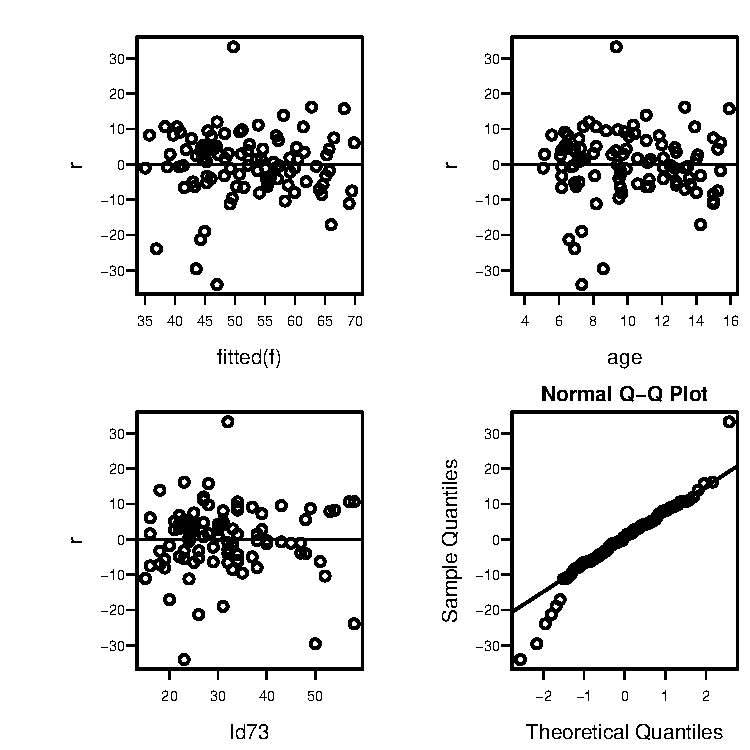
\includegraphics[width=\maxwidth]{rmsintro-unnamed-chunk-7-1} }

\end{Schunk}
\ei

\section{Plotting Partial Effects}\sound{rrms-6}
\bi
\item \co{Predict} and \co{ggplot} makes one plot for each predictor
\item Predictor is on $x$-axis, $\hat{y}$ on the $y$-axis
\item Predictors not shown in plot are set to constants
 \bi
 \item median for continuous predictors
 \item mode for categorical ones
 \ei
\item For categorical predictor, estimates are shown only at data
  values
\item 0.95 pointwise confidence limits for $\hat{E}(y|x)$ are shown
  (add \co{conf.int=FALSE} to \co{Predict()} to suppress CLs)
\item Example: \ipacue
\begin{Schunk}
\begin{Sinput}
ggplot(Predict(f))
\end{Sinput}


\centerline{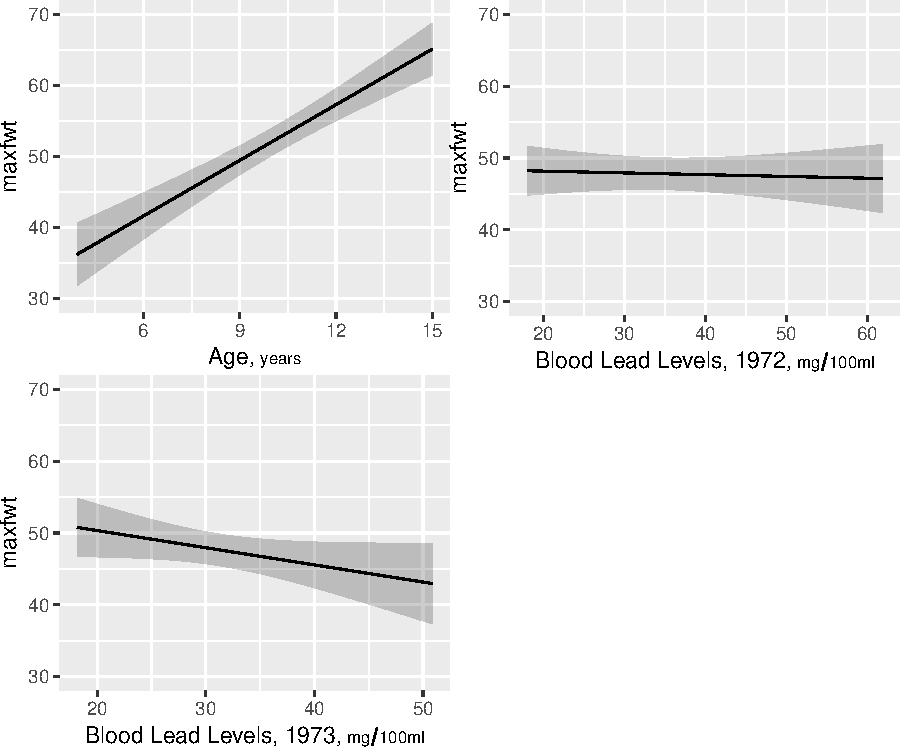
\includegraphics[width=\maxwidth]{rmsintro-unnamed-chunk-8-1} }

\end{Schunk}
\item To take control of which predictors are plotted, or to specify
  customized options: \ipacue
\begin{Schunk}
\begin{Sinput}
ggplot(Predict(f, age))   # plot age effect, using default range,
                          # 10th smallest to 10th largest age
\end{Sinput}


\centerline{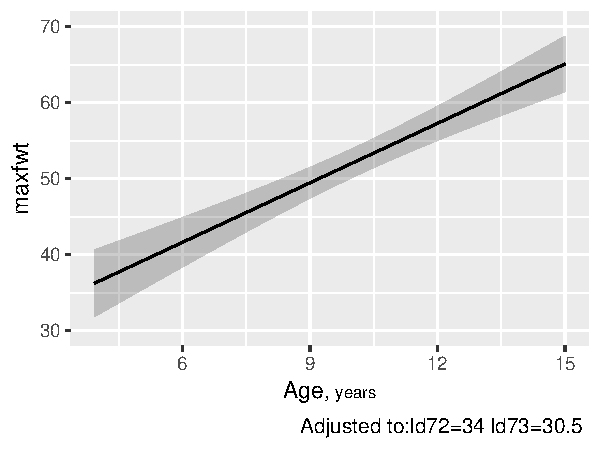
\includegraphics[width=\maxwidth]{rmsintro-unnamed-chunk-9-1} }

\end{Schunk}
\begin{Schunk}
\begin{Sinput}
ggplot(Predict(f, age=3:15))  # plot age=3,4,...,15 (*\ipacue*)
\end{Sinput}


\centerline{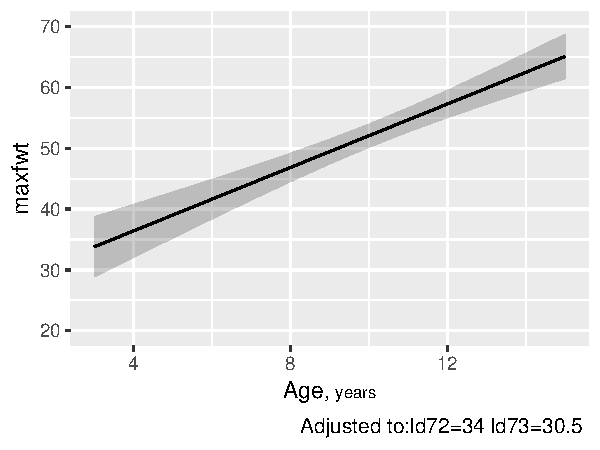
\includegraphics[width=\maxwidth]{rmsintro-unnamed-chunk-10-1} }

\end{Schunk}
\begin{Schunk}
\begin{Sinput}
ggplot(Predict(f, age=seq(3,16,length=150)))   # plot age=3-16, 150 points (*\ipacue*)
\end{Sinput}


\centerline{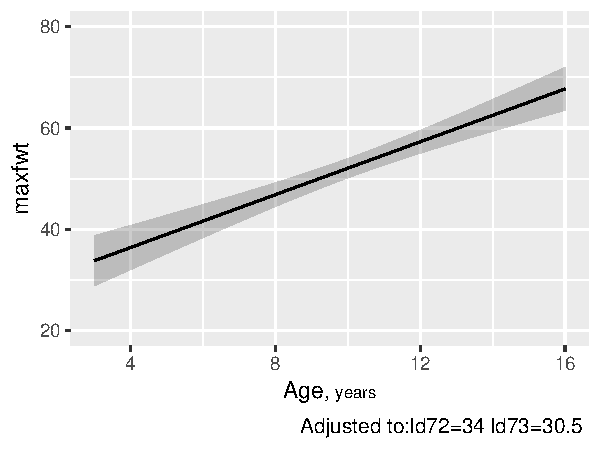
\includegraphics[width=\maxwidth]{rmsintro-unnamed-chunk-11-1} }

\end{Schunk}
\item To get confidence limits for $\hat{y}$: \ipacue
\begin{Schunk}
\begin{Sinput}
ggplot(Predict(f, age, conf.type='individual'))
\end{Sinput}


\centerline{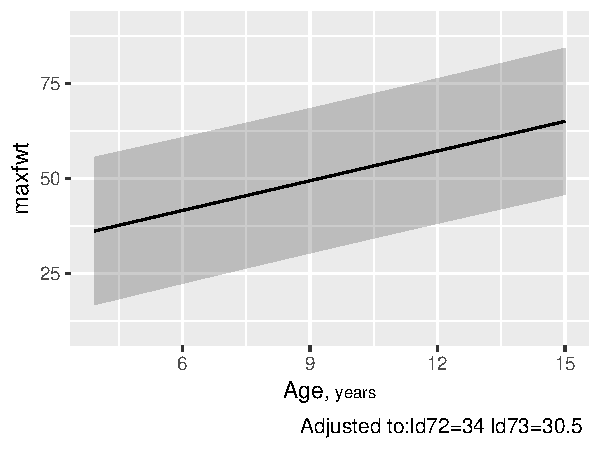
\includegraphics[width=\maxwidth]{rmsintro-unnamed-chunk-12-1} }

\end{Schunk}
\item To show both types of 0.99 confidence limits on one plot: \ipacue
\begin{Schunk}
\begin{Sinput}
p1 <- Predict(f, age, conf.int=0.99, conf.type='individual')
p2 <- Predict(f, age, conf.int=0.99, conf.type='mean')
p <- rbind(Individual=p1, Mean=p2)
ggplot(p)
\end{Sinput}


\centerline{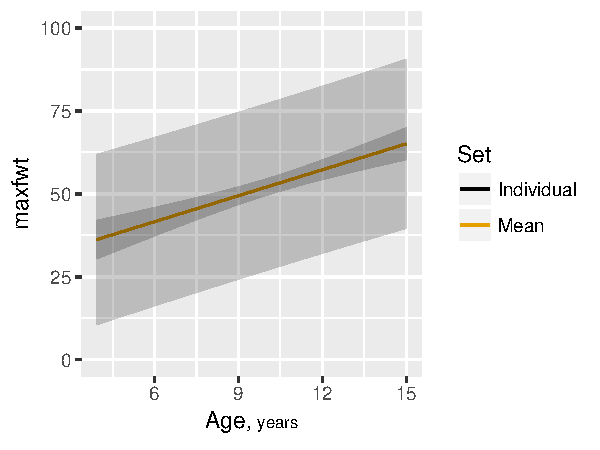
\includegraphics[width=\maxwidth]{rmsintro-unnamed-chunk-13-1} }

\end{Schunk}
\item Non-plotted variables are set to reference values (median and
  mode by default)
\item To control the settings of non-plotted values use e.g. \ipacue
\begin{Schunk}
\begin{Sinput}
ggplot(Predict(f, ld73, age=3))
\end{Sinput}


\centerline{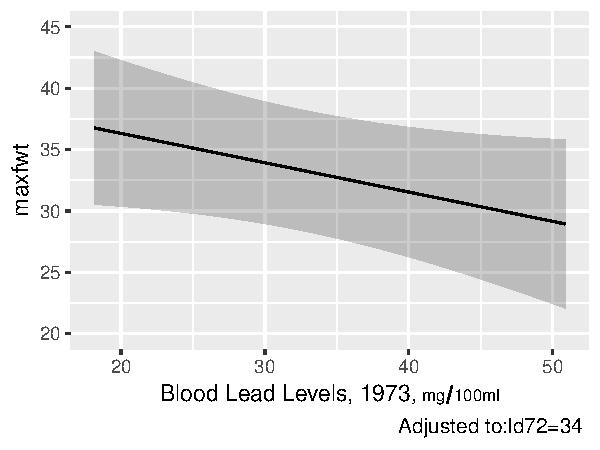
\includegraphics[width=\maxwidth]{rmsintro-unnamed-chunk-14-1} }

\end{Schunk}
\item To make separate lines for two ages: \ipacue
\begin{Schunk}
\begin{Sinput}
ggplot(Predict(f, ld73, age=c(3,9)))  # add ,conf.int=FALSE to suppress conf. bands
\end{Sinput}


\centerline{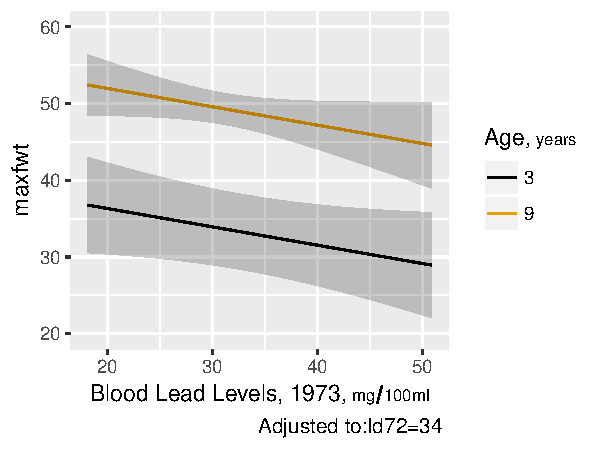
\includegraphics[width=\maxwidth]{rmsintro-unnamed-chunk-15-1} }

\end{Schunk}
\item To plot a 3-d surface for two continuous predictors against
  $\hat{y}$; color coding for predicted mean \co{maxfwt} \ipacue
\begin{Schunk}
\begin{Sinput}
bplot(Predict(f, ld72, ld73))
\end{Sinput}


\centerline{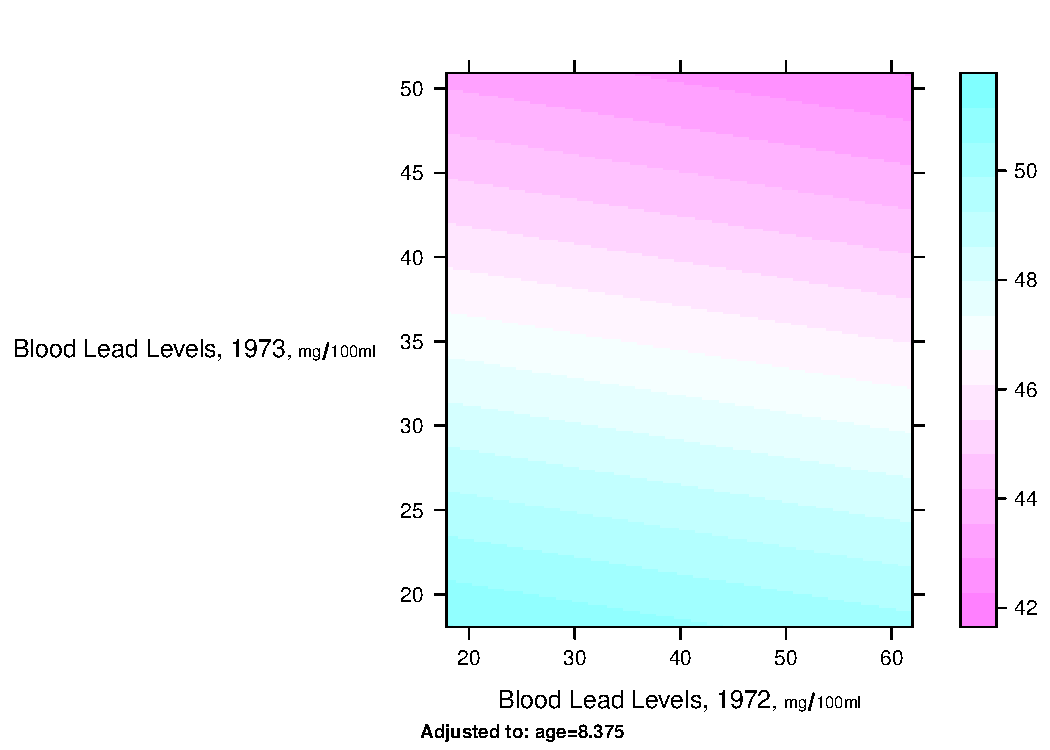
\includegraphics[width=\maxwidth]{rmsintro-unnamed-chunk-16-1} }

\end{Schunk}
\ei

\section{Nomograms: Overall Depiction of Fitted Models} \sound{rrms-7}\ipacue
\begin{Schunk}
\begin{Sinput}
plot(nomogram(f))
\end{Sinput}


\centerline{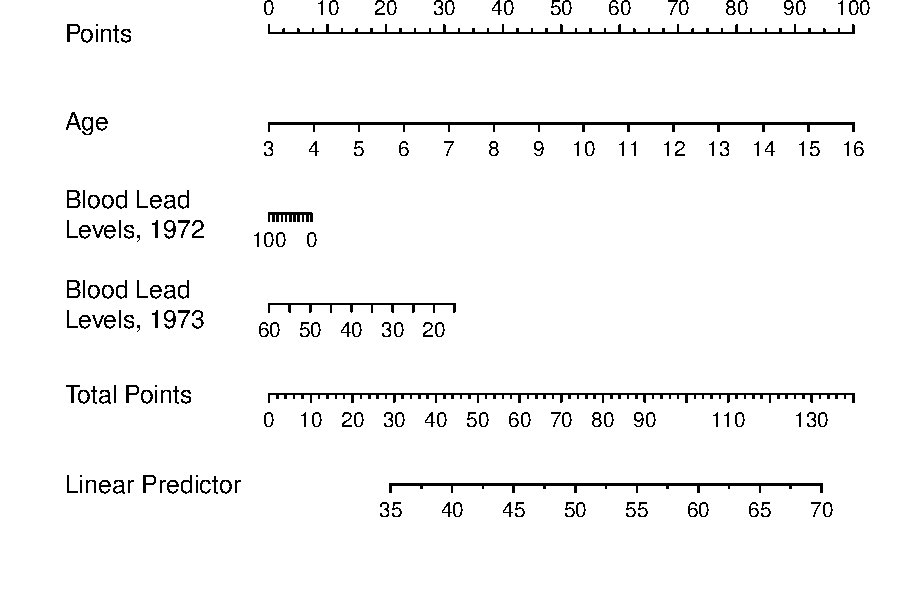
\includegraphics[width=\maxwidth]{rmsintro-unnamed-chunk-17-1} }

\end{Schunk}
See \href{http://stats.stackexchange.com/questions/155430/clarifications-regarding-reading-a-nomogram}{this}
for excellent examples showing how to read such nomograms.

\subsection{Point Estimates for Partial Effects} \sound{rrms-8}\ipacue
The \co{summary} function can compute point estimates and confidence
intervals for effects of individual predictors, holding other
predictors to selected constants.  The constants you hold other
predictors to will only matter when the other predictors interact with
the predictor whose effects are being displayed.

How predictors are changed depend on the type of predictor:
\bi
\item Categorical predictors: differences against the reference (most
  frequent) cell by default
\item Continuous predictors: inter-quartile-range effects by default
\ei
The estimated effects depend on the type of model:
\bi
\item \co{ols}: differences in means
\item logistic models: odds ratios and their logs
\item Cox models: hazard ratios and their logs
\item quantile regression: differences in quantiles
\ei

\begin{Schunk}
\begin{Sinput}
summary(f)         # inter-quartile-range effects (*\ipacue*)
\end{Sinput}
\begin{Soutput}
             Effects              Response : maxfwt 

 Factor Low     High   Diff.   Effect   S.E.   Lower 0.95 Upper 0.95
 age     6.1667 12.021  5.8542 15.26700 1.8914 11.5120    19.02200  
 ld72   27.0000 43.000 16.0000 -0.39356 1.2511 -2.8773     2.09010  
 ld73   24.0000 37.000 13.0000 -3.10660 1.7222 -6.5255     0.31234  
\end{Soutput}
\begin{Sinput}
summary(f, age=5)  # adjust age to 5 when examining ld72,ld73
\end{Sinput}
\begin{Soutput}
             Effects              Response : maxfwt 

 Factor Low     High   Diff.   Effect   S.E.   Lower 0.95 Upper 0.95
 age     6.1667 12.021  5.8542 15.26700 1.8914 11.5120    19.02200  
 ld72   27.0000 43.000 16.0000 -0.39356 1.2511 -2.8773     2.09010  
 ld73   24.0000 37.000 13.0000 -3.10660 1.7222 -6.5255     0.31234  
\end{Soutput}
\begin{Sinput}
                   # (no effect since no interactions in model)
summary(f, ld73=c(20, 40))  # effect of changing ld73 from 20 to 40
\end{Sinput}
\begin{Soutput}
             Effects              Response : maxfwt 

 Factor Low     High   Diff.   Effect   S.E.   Lower 0.95 Upper 0.95
 age     6.1667 12.021  5.8542 15.26700 1.8914  11.5120   19.02200  
 ld72   27.0000 43.000 16.0000 -0.39356 1.2511  -2.8773    2.09010  
 ld73   20.0000 40.000 20.0000 -4.77940 2.6495 -10.0390    0.48052  
\end{Soutput}
\end{Schunk}

When a predictor has a linear effect, its slope is the one-unit change
in $Y$ when the predictor increases by one unit.  So the following
trick can be used to get a confidence interval for a slope: use
\co{summary} to get the confidence interval for the one-unit change:

\begin{Schunk}
\begin{Sinput}
summary(f, age=5:6)    # starting age irrelevant since age is linear (*\ipacue*)
\end{Sinput}
\begin{Soutput}
             Effects              Response : maxfwt 

 Factor Low High Diff. Effect   S.E.    Lower 0.95 Upper 0.95
 age     5   6    1     2.60780 0.32308  1.9664    3.24920   
 ld72   27  43   16    -0.39356 1.25110 -2.8773    2.09010   
 ld73   24  37   13    -3.10660 1.72220 -6.5255    0.31234   
\end{Soutput}
\end{Schunk}

There is a \co{plot} method for \co{summary} results.  By default it
shows 0.9, 0.95, and 0.99 confidence limits. \ipacue
\begin{Schunk}
\begin{Sinput}
plot(summary(f))
\end{Sinput}


\centerline{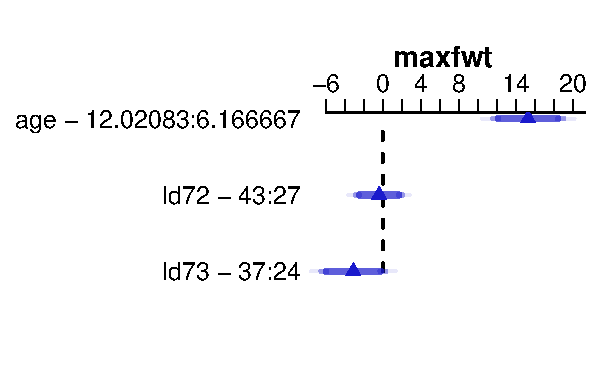
\includegraphics[width=\maxwidth]{rmsintro-unnamed-chunk-20-1} }

\end{Schunk}

\section{Getting Predicted Values}\sound{rrms-9}
\bi
\item Using \co{predict}
\begin{Schunk}
\begin{Sinput}
predict(f, data.frame(age=3, ld72=21, ld73=21))
\end{Sinput}
\begin{Soutput}
       1 
36.39448 
\end{Soutput}
\begin{Sinput}
# must specify all variables in the model

predict(f, data.frame(age=c(3, 10), ld72=21, ld73=c(21, 47)))
\end{Sinput}
\begin{Soutput}
       1        2 
36.39448 48.43618 
\end{Soutput}
\begin{Sinput}
# predictions for (3,21,21) and (10,21,47)

newdat <- expand.grid(age=c(4, 8), ld72=c(21, 47), ld73=c(21, 47))
newdat
\end{Sinput}
\begin{Soutput}
  age ld72 ld73
1   4   21   21
2   8   21   21
3   4   47   21
4   8   47   21
5   4   21   47
6   8   21   47
7   4   47   47
8   8   47   47
\end{Soutput}
\begin{Sinput}
predict(f, newdat)     # 8 predictions
\end{Sinput}
\begin{Soutput}
       1        2        3        4        5        6        7        8 
39.00232 49.43370 38.36278 48.79416 32.78911 43.22049 32.14957 42.58095 
\end{Soutput}
\begin{Sinput}
predict(f, newdat, conf.int=0.95)  # also get CLs for mean (*\ipacue*)
\end{Sinput}
\begin{Soutput}
$linear.predictors
       1        2        3        4        5        6        7        8 
39.00232 49.43370 38.36278 48.79416 32.78911 43.22049 32.14957 42.58095 

$lower
       1        2        3        4        5        6        7        8 
33.97441 46.23595 32.15468 43.94736 25.68920 36.94167 27.17060 38.86475 

$upper
       1        2        3        4        5        6        7        8 
44.03023 52.63145 44.57088 53.64095 39.88902 49.49932 37.12854 46.29716 
\end{Soutput}
\begin{Sinput}
predict(f, newdat, conf.int=0.95, conf.type='individual')  # CLs for indiv.
\end{Sinput}
\begin{Soutput}
$linear.predictors
       1        2        3        4        5        6        7        8 
39.00232 49.43370 38.36278 48.79416 32.78911 43.22049 32.14957 42.58095 

$lower
       1        2        3        4        5        6        7        8 
19.44127 30.26132 18.46566 29.27888 12.59596 23.30120 12.60105 23.31531 

$upper
       1        2        3        4        5        6        7        8 
58.56337 68.60609 58.25989 68.30944 52.98227 63.13979 51.69810 61.84659 
\end{Soutput}
\end{Schunk}
See also \co{gendata}.
\item The brute-force way
\begin{Schunk}
\begin{Sinput}
# Model is b1 + b2*age + b3*ld72 + b4*ld73
b <- coef(f)
# For 3 year old with both lead exposures 21
b[1] + b[2]*3 + b[3]*21 + b[4]*21
\end{Sinput}
\begin{Soutput}
Intercept 
 36.39448 
\end{Soutput}
\end{Schunk}
\item Using \co{Function} function \ipacue
\begin{Schunk}
\begin{Sinput}
g <- Function(f)
g(age=c(3, 8), ld72=21, ld73=21)       # 2 predictions
\end{Sinput}
\begin{Soutput}
[1] 36.39448 49.43370
\end{Soutput}
\begin{Sinput}
g(age=3)              # 3 year old at median ld72, ld73
\end{Sinput}
\begin{Soutput}
[1] 33.80449
\end{Soutput}
\end{Schunk}
\ei

\section{ANOVA}\sound{rrms-10}
\bi
\item Use \co{anova(fitobject)} to get all total effects and
  individual partial effects
\item Use \co{anova(f,age,sex)} to get combined partial effects of
  \co{age} and \co{sex}, for example
\item Store result of \co{anova} in an object in you want to print it
  various ways, or to plot it:
\begin{Schunk}
\begin{Sinput}
an <- anova(f)
an                     # same as print(an)
\end{Sinput}
\begin{Soutput}
                Analysis of Variance          Response: maxfwt 

 Factor     d.f. Partial SS  MS          F     P     
 age         1   5907.535742 5907.535742 65.15 <.0001
 ld72        1      8.972994    8.972994  0.10 0.7538
 ld73        1    295.044370  295.044370  3.25 0.0744
 REGRESSION  3   7540.087710 2513.362570 27.72 <.0001
 ERROR      95   8613.750674   90.671060             
\end{Soutput}
\begin{Sinput}
print(an, 'names')     # print names of variables being tested
\end{Sinput}
\begin{Soutput}
                Analysis of Variance          Response: maxfwt 

 Factor     d.f. Partial SS  MS          F     P      Tested       
 age         1   5907.535742 5907.535742 65.15 <.0001 age          
 ld72        1      8.972994    8.972994  0.10 0.7538 ld72         
 ld73        1    295.044370  295.044370  3.25 0.0744 ld73         
 REGRESSION  3   7540.087710 2513.362570 27.72 <.0001 age,ld72,ld73
 ERROR      95   8613.750674   90.671060                           
\end{Soutput}
\begin{Sinput}
print(an, 'subscripts')# print subscripts in coef(f) (ignoring (*\ipacue*)
\end{Sinput}
\begin{Soutput}
                Analysis of Variance          Response: maxfwt 

 Factor     d.f. Partial SS  MS          F     P      Tested
 age         1   5907.535742 5907.535742 65.15 <.0001 1     
 ld72        1      8.972994    8.972994  0.10 0.7538 2     
 ld73        1    295.044370  295.044370  3.25 0.0744 3     
 REGRESSION  3   7540.087710 2513.362570 27.72 <.0001 1-3   
 ERROR      95   8613.750674   90.671060                    

Subscripts correspond to:
[1] age  ld72 ld73
\end{Soutput}
\begin{Sinput}
                       # the intercept) being tested
print(an, 'dots')      # a dot in each position being tested
\end{Sinput}
\begin{Soutput}
                Analysis of Variance          Response: maxfwt 

 Factor     d.f. Partial SS  MS          F     P      Tested
 age         1   5907.535742 5907.535742 65.15 <.0001 .     
 ld72        1      8.972994    8.972994  0.10 0.7538  .    
 ld73        1    295.044370  295.044370  3.25 0.0744   .   
 REGRESSION  3   7540.087710 2513.362570 27.72 <.0001 ...   
 ERROR      95   8613.750674   90.671060                    

Subscripts correspond to:
[1] age  ld72 ld73
\end{Soutput}
\begin{Sinput}
anova(f, ld72, ld73)   # combine effects into a 2 d.f. test (*\ipacue*)
\end{Sinput}
\begin{Soutput}
                Analysis of Variance          Response: maxfwt 

 Factor     d.f. Partial SS  MS         F    P     
 ld72        1      8.972994   8.972994 0.10 0.7538
 ld73        1    295.044370 295.044370 3.25 0.0744
 REGRESSION  2    747.283558 373.641779 4.12 0.0192
 ERROR      95   8613.750674  90.671060            
\end{Soutput}
\end{Schunk}
\ei
\def\apacue{0}
